\input templates/header
\title[ASD - Scelta struttura dati]{\textbf{Algoritmi e Strutture Dati}\\[24pt]Scelta della struttura dati}

\renewcommand{\Primo}{\mathit{start}\xspace}
\renewcommand{\Ultimo}{\mathit{end}\xspace}

\usepackage{tikz}
\usetikzlibrary{trees}
\usetikzlibrary{matrix}
\usetikzlibrary{graphs}
\usetikzlibrary{shapes}
\usetikzlibrary{positioning}
\usepackage{xmpmulti}
\usepackage{listings}

\lstset{
  basicstyle=\ttfamily,
  columns=fullflexible,
  keywordstyle=\color{red}\bfseries,
  commentstyle=\color{blue},
  showstringspaces=false,
}

\definecolor{ocra}{rgb}{1.0,0.9,0.7}

\tikzset{
    Node/.style = {circle, draw=black, align=center, fill=yellow!20, thick}
}	
\tikzset{
    Edge/.style = {draw=black,thick,-latex}
}	


\graphicspath{{figs/11/}}

\begin{document}

%-------------------------------------------------------------------------
\FrameTitle{}

%-------------------------------------------------------------------------
\FrameContent



%%%%%%%%%%%%%%%%%%%%%%%%%%%%%%%%%%%%%%%%%%%%%%%%%%%%%%%%%%%%%%%%%%%%%%%%%%
\section{Introduzione}

%-------------------------------------------------------------------------
\begin{frame}{Problema cammini minimi}

\vspace{-6	pt}
\begin{block}{Input}
\BI
\item \alert{Grafo orientato} $G=(V,E)$
\item Un nodo \alert{sorgente} $s$
\item Una \alert{funzione di peso} $w: E \rightarrow R$
\EI
\end{block}

\begin{block}{Definizione}
\smallskip
\TwoColsCustom{0.60}{0.36}{
\smallskip
Dato un cammino $p = \langle v_1, v_2, \ldots, v_k \rangle$ con $k > 1$, il \alert{costo del cammino} è dato da
}{\[
w(p) = \sum_{i=2}^k w(v_{i-1},v_i)
\]
}
\end{block}

\begin{block}{Output}
Trovare un cammino da $s$ ad $u$, per ogni nodo $u \in V$ , il cui costo sia minimo, ovvero più 
piccolo o uguale del costo di qualunque altro cammino da $s$ a $u$.
\end{block}

\end{frame}

\begin{frame}[shrink=5]{Panoramica sul problema}
\BB{Cammini minimi da sorgente unica}
\BI
\item \alert{Input}: Grafo pesato, nodo radice $s$ 
\item \alert{Output}: i cammini minimi che vanno da $s$ a tutti gli altri nodi $v$
\EI

\BB{Cammino minimo tra una coppia di vertici}
\BI
\item \alert{Input}: Grafo pesato, una coppia di vertici $s$, $d$
\item \alert{Output}: un cammino minimo fra $s$ e $d$
\item Si risolve il primo problema e si estrae il cammino richiesto. 
Non si conoscono algoritmi che abbiano tempo di esecuzione migliore.
\EI

\BB{Cammini mimimi tra tutte le coppie di vertici} 
\BI
\item \alert{Input}: Grafo pesato
\item \alert{Output}: i cammini minimi fra tutte le coppie di vertici. 
\item Soluzione basata su programmazione dinamica		
\EI
\end{frame}

%-------------------------------------------------------------------------
\begin{frame}{Pesi}

\begin{columns}[T]
\column{0.63\textwidth}
\BB{Tipologie di pesi}
Algoritmi diversi possono funzionare oppure no in caso di alcune categorie speciali di pesi
\BIL
\item Positivi / positivi+negativi
\item Reali / interi
\EIL

\bigskip
\BB{Pesi negativi vs grafi con cicli negativi}
Esempio: proprietario di un TIR
\BIL
\item Viaggare scarico: perdita, peso positivo
\item Viaggare carico: profitto, peso negativo
\EIL
\column{0.35\textwidth}

\vspace{-12pt}
\begin{center}
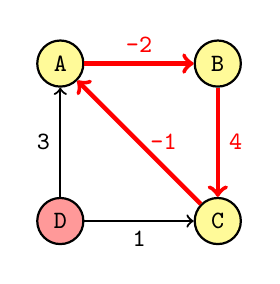
\begin{tikzpicture}[
    thick,
    font=\ttfamily\bfseries\small
]
\tikzset{
    mynode/.style = {circle, draw=black, align=center,fill=yellow!40},
    mynoder/.style = {circle, draw=black, align=center,fill=red!40},
    edgen/.style = {->,thick},
    edger/.style = {->,ultra thick,red}
}
\node[mynode] at (0.0,2.0) (a) {A};
\node[mynode] at (2.0,2.0) (b) {B};
\node[mynode] at (2.0,0.0) (c) {C};
\node[mynoder] at (0.0,0.0) (d) {D};
\draw[edger] (a) edge node[above] {-2} (b);
\draw[edger] (b) edge node[right] {4} (c);
\draw[edger] (c) edge node[right] {-1} (a);
\draw[edgen] (d) edge node[below] {1} (c);
\draw[edgen] (d) edge node[left] {3} (a);
\end{tikzpicture}
\end{center}

\begin{center}
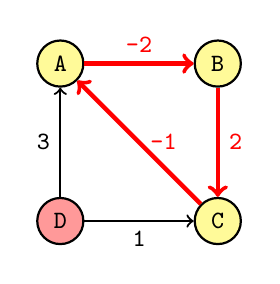
\begin{tikzpicture}[
    thick,
    font=\ttfamily\bfseries\small
]
\tikzset{
    mynode/.style = {circle, draw=black, align=center,fill=yellow!40},
    mynoder/.style = {circle, draw=black, align=center,fill=red!40},
    edgen/.style = {->,thick},
    edger/.style = {->,ultra thick,red}
}
\node[mynode] at (0.0,2.0) (a) {A};
\node[mynode] at (2.0,2.0) (b) {B};
\node[mynode] at (2.0,0.0) (c) {C};
\node[mynoder] at (0.0,0.0) (d) {D};
\draw[edger] (a) edge node[above] {-2} (b);
\draw[edger] (b) edge node[right] {2} (c);
\draw[edger] (c) edge node[right] {-1} (a);
\draw[edgen] (d) edge node[below] {1} (c);
\draw[edgen] (d) edge node[left] {3} (a);
\end{tikzpicture}
\end{center}

\end{columns}

\end{frame}

\section{Cammini minimi, sorgente singola}


%-------------------------------------------------------------------------
\begin{frame}[fragile]{Problema cammini minimi -- Sottostruttura ottima}

\TwoCols{
\medskip
Si noti che due cammini minimi possono avere un tratto in comune $A \leadsto B$ \ldots
}{
\vspace{-12pt}
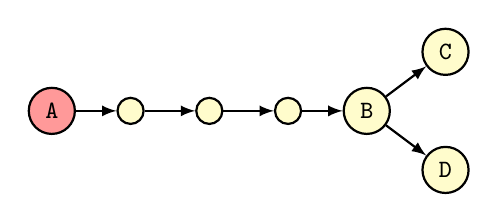
\begin{tikzpicture}[
    thick,
    font=\ttfamily\bfseries\small
]
\tikzset{
    mynoder/.style = {circle, draw=black, align=center,fill=red!40},
}
\node[mynoder] at (0,0) (A) {A};
\node[Node] at (1,0) (u1) {};
\node[Node] at (2,0) (u2) {};
\node[Node] at (3,0) (u3) {};
\node[Node] at (4,0) (B) {B};
\node[Node] at (5,0.75) (C) {C};
\node[Node] at (5,-0.75) (D) {D};
\path (A) edge [Edge] (u1);
\path (u1) edge [Edge] (u2);
\path (u2) edge [Edge] (u3);
\path (u3) edge [Edge] (B);
\path (B) edge [Edge] (C);
\path (B) edge [Edge] (D);
\end{tikzpicture}
}

\TwoCols{
\bigskip
\ldots ma non possono convergere in un nodo comune $B$ dopo aver percorso un tratto iniziale distinto 
}{
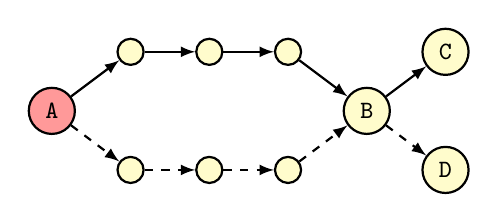
\begin{tikzpicture}[
    thick,
    font=\ttfamily\bfseries\small
]
\tikzset{
    mynoder/.style = {circle, draw=black, align=center,fill=red!40},
}

\node[mynoder] at (0,0) (A) {A};
\node[Node] at (1,0.75) (u1) {};
\node[Node] at (2,0.75) (u2) {};
\node[Node] at (3,0.75) (u3) {};
\node[Node] at (1,-0.75) (d1) {};
\node[Node] at (2,-0.75) (d2) {};
\node[Node] at (3,-0.75) (d3) {};
\node[Node] at (4,0) (B) {B};
\node[Node] at (5,0.75) (C) {C};
\node[Node] at (5,-0.75) (D) {D};
\path (A) edge [Edge] (u1);
\path (u1) edge [Edge] (u2);
\path (u2) edge [Edge] (u3);
\path (u3) edge [Edge] (B);
\path (A) edge [Edge,dashed] (d1);
\path (d1) edge [Edge,dashed] (d2);
\path (d2) edge [Edge,dashed] (d3);
\path (d3) edge [Edge,dashed] (B);
\path (B) edge [Edge] (C);
\path (B) edge [Edge,dashed] (D);
\end{tikzpicture}
}

\begin{block}{Albero dei cammini minimi}
L'\alert{albero dei cammini minimi} è un albero di copertura radicato in $s$ avente un cammino da $s$ a tutti i nodi raggiungibili da $s$.
\end{block}

\end{frame}

%-------------------------------------------------------------------------
\begin{frame}{Soluzione ammissibile}

\begin{block}{Soluzione ammissibile}
Una soluzione \alert{ammissibile} può essere descritta da un \alert{albero di copertura $T$}
radicato in $s$ e da un \alert{vettore di distanza $d$}, \\
i cui valori $d[u]$ rappresentano il costo del cammino da $s$ a $u$ in $T$.
\end{block}

\bigskip
\small
\begin{center}
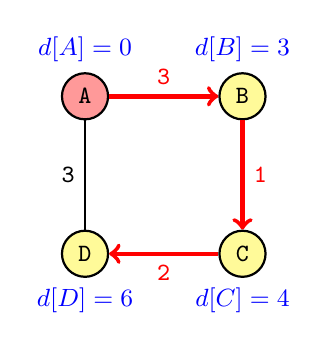
\begin{tikzpicture}[
    thick,
    font=\ttfamily\bfseries\small
]
\tikzset{
    mynode/.style = {circle, draw=black, align=center,fill=yellow!40},
    mynoder/.style = {circle, draw=black, align=center,fill=red!40},
    edgen/.style = {-},
    edger/.style = {->,ultra thick,red}
}
\node[mynoder, label={above:{\color{blue} $d[A]=0$}}] at (0.0,2.0) (a) {A};
\node[mynode,  label={above:{\color{blue} $d[B]=3$}}] at (2.0,2.0) (b) {B};
\node[mynode,  label={below:{\color{blue} $d[C]=4$}}] at (2.0,0.0) (c) {C};
\node[mynode,  label={below:{\color{blue} $d[D]=6$}}] at (0.0,0.0) (d) {D};
\draw[edger] (a) edge node[above] {3} (b);
\draw[edger] (b) edge node[right] {1} (c);
\draw[edger] (c) edge node[below] {2} (d);
\draw[edgen] (d) edge node[left] {3} (a);
\end{tikzpicture}
\qquad
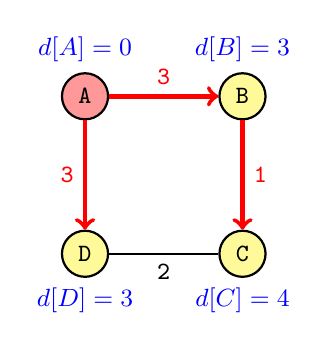
\begin{tikzpicture}[
    thick,
    font=\ttfamily\bfseries\small
]
\tikzset{
    mynode/.style = {circle, draw=black, align=center,fill=yellow!40},
    mynoder/.style = {circle, draw=black, align=center,fill=red!40},
    edgen/.style = {-},
    edger/.style = {->,ultra thick,red}
}
\node[mynoder, label={above:{\color{blue} $d[A]=0$}}] at (0.0,2.0) (a) {A};
\node[mynode,  label={above:{\color{blue} $d[B]=3$}}] at (2.0,2.0) (b) {B};
\node[mynode,  label={below:{\color{blue} $d[C]=4$}}] at (2.0,0.0) (c) {C};
\node[mynode,  label={below:{\color{blue} $d[D]=3$}}] at (0.0,0.0) (d) {D};
\draw[edger] (a) edge node[above] {3} (b);
\draw[edger] (b) edge node[right] {1} (c);
\draw[edgen] (c) edge node[below] {2} (d);
\draw[edger] (a) edge node[left] {3} (d);
\end{tikzpicture}


\end{center}

\end{frame}

\begin{frame}{Cammini minimi / alberi di copertura di peso minimo}

\BB{Questi due alberi di copertura sono identici?}
\BI
\item un \alert<2>{albero dei cammini minimi} da singola sorgente $A$
\item un \alert<3>{albero di copertura di peso minimo}
\EI

\bigskip
\centering
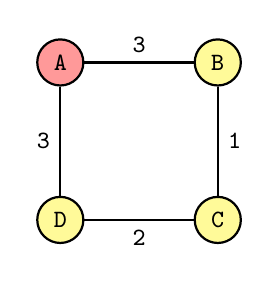
\begin{tikzpicture}[
    thick,
    font=\ttfamily\bfseries\small
]
\tikzset{
    mynode/.style = {circle, draw=black, align=center,fill=yellow!40},
    mynoder/.style = {circle, draw=black, align=center,fill=red!40},
    edgen/.style = {-},
    edger/.style = {-,ultra thick,red}
}
\node[mynode] at (0.0,0.0) (d) {D};
\node[mynoder] at (0.0,2.0) (a) {A};
\node[mynode] at (2.0,2.0) (b) {B};
\node[mynode] at (2.0,0.0) (c) {C};
\draw[edgen] (a) edge node[above] {3} (b);
\draw[edgen] (b) edge node[right] {1} (c);
\draw[edgen] (c) edge node[below] {2} (d);
\draw[edgen] (a) edge node[left] {3} (d);
\end{tikzpicture}
\qquad\pause
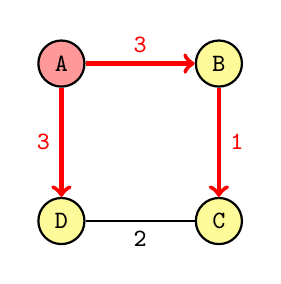
\begin{tikzpicture}[
    thick,
    font=\ttfamily\bfseries\small
]
\tikzset{
    mynode/.style = {circle, draw=black, align=center,fill=yellow!40},
    mynoder/.style = {circle, draw=black, align=center,fill=red!40},
    edgen/.style = {-},
    edger/.style = {->,ultra thick,red}
}
\node[mynode] at (0.0,0.0) (d) {D};
\node[mynoder] at (0.0,2.0) (a) {A};
\node[mynode] at (2.0,2.0) (b) {B};
\node[mynode] at (2.0,0.0) (c) {C};
\draw[edger] (a) edge node[above] {3} (b);
\draw[edger] (b) edge node[right] {1} (c);
\draw[edgen] (c) edge node[below] {2} (d);
\draw[edger] (a) edge node[left] {3} (d);
\end{tikzpicture}
\qquad\pause
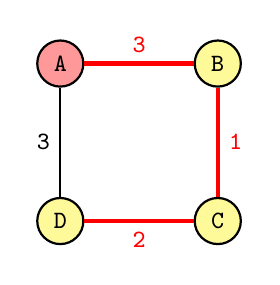
\begin{tikzpicture}[
    thick,
    font=\ttfamily\bfseries\small
]
\tikzset{
    mynode/.style = {circle, draw=black, align=center,fill=yellow!40},
    mynoder/.style = {circle, draw=black, align=center,fill=red!40},
    edgen/.style = {-},
    edger/.style = {-,ultra thick,red}
}
\node[mynode] at (0.0,0.0) (d) {D};
\node[mynoder] at (0.0,2.0) (a) {A};
\node[mynode] at (2.0,2.0) (b) {B};
\node[mynode] at (2.0,0.0) (c) {C};
\draw[edger] (a) edge node[above] {3} (b);
\draw[edger] (b) edge node[right] {1} (c);
\draw[edger] (c) edge node[below] {2} (d);
\draw[edgen] (d) edge node[left] {3} (a);
\end{tikzpicture}

\end{frame}

\begin{frame}{Rappresentazione albero}

Per rappresentare l'albero, utilizziamo la rappresentazione basata su vettore dei padri,
così come abbiamo fatto con le visite in ampiezza/profondità.

\bigskip
\begin{Procedure}
\caption[A]{\textsf{printPath}($\Node\ s,\ \Node\ d,\ \Node[\,]\ T$)}

\uIf{$s == d$}
{
  \textbf{print} $s$
}
\uElseIf{$\parent[d] == \Nil$}
{
  \textbf{print} “error”\;
}
\Else
{
  $\textsf{printPath}(s, T[d], T)$\;
  \textbf{print} $d$
}
\end{Procedure}

\end{frame}



\begin{frame}{Teorema di Bellman}

\vspace{-12pt}
\begin{block}{Teorema di Bellman}
Una soluzione ammissibile $T$ è \alert{ottima} se e solo se:
\begin{align*} 
d[v] = d[u] + w(u,v) && \textrm{per ogni arco $(u,v) \in T$}\\
d[v] \leq d[u] + w(u,v) && \textrm{per ogni arco $(u,v) \in E$}
\end{align*}
\end{block}

\vspace{-21pt}
\begin{columns}[T]
\column{0.45\textwidth}
\begin{center}
\begingroup
\tiny
\begin{align*}
d[B] = d[A] + w(A,B)  &\quad
d[C] = d[B] + w(B,C)\\
d[D] = d[C] + w(C,D)  &\quad
\alert{d[D] > d[A] + w(A,D)}
\end{align*}
\endgroup
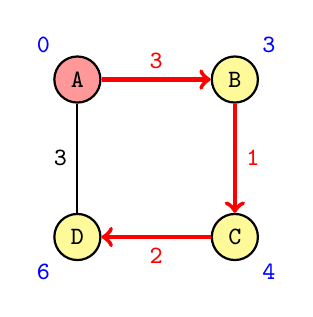
\begin{tikzpicture}[
    thick,
    font=\ttfamily\bfseries\small
]
\tikzset{
    mynode/.style = {circle, draw=black, align=center,fill=yellow!40},
    mynoder/.style = {circle, draw=black, align=center,fill=red!40},
    edgen/.style = {-},
    edger/.style = {->,ultra thick,red}
}
\node[mynoder, label={above left:{\color{blue} 0}}] at (0.0,2.0) (a) {A};
\node[mynode, label={above right:{\color{blue} 3}}] at (2.0,2.0) (b) {B};
\node[mynode, label={below right:{\color{blue} 4}}] at (2.0,0.0) (c) {C};
\node[mynode, label={below left:{\color{blue} 6}}] at (0.0,0.0) (d) {D};
\draw[edger] (a) edge node[above] {3} (b);
\draw[edger] (b) edge node[right] {1} (c);
\draw[edger] (c) edge node[below] {2} (d);
\draw[edgen] (d) edge node[left] {3} (a);
\end{tikzpicture}
\end{center}

\column{0.45\textwidth}
\begin{center}
\begingroup
\tiny
\begin{align*}
d[B] = d[A] + w(A,B) &\quad
d[C] = d[B] + w(B,C)\\
d[D] = d[A] + w(A,D) &\quad
d[D] \leq d[C] + w(C,D)
\end{align*}
\endgroup
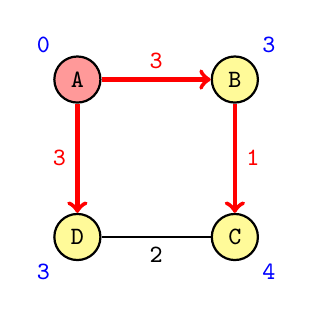
\begin{tikzpicture}[
    thick,
    font=\ttfamily\bfseries\small
]
\tikzset{
    mynode/.style = {circle, draw=black, align=center,fill=yellow!40},
    mynoder/.style = {circle, draw=black, align=center,fill=red!40},
    edgen/.style = {-},
    edger/.style = {->,ultra thick,red}
}
\node[mynoder, label={above left:{\color{blue} 0}}] at (0.0,2.0) (a) {A};
\node[mynode, label={above right:{\color{blue} 3}}] at (2.0,2.0) (b) {B};
\node[mynode, label={below right:{\color{blue} 4}}] at (2.0,0.0) (c) {C};
\node[mynode, label={below left:{\color{blue} 3}}] at (0.0,0.0) (d) {D};
\draw[edger] (a) edge node[above] {3} (b);
\draw[edger] (b) edge node[right] {1} (c);
\draw[edgen] (c) edge node[below] {2} (d);
\draw[edger] (a) edge node[left] {3} (d);
\end{tikzpicture}
\end{center}

\end{columns}


\end{frame}

%-------------------------------------------------------------------------
\begin{frame}{Dimostrazione}

\begin{block}{Teorema di Bellman - Parte 1}
Se $T$ è una soluzione ottima, allora valgono le condizioni di Bellman:
\begin{align*} 
d[v] = d[u] + w(u,v) && \textrm{per ogni arco $(u,v) \in T$}\\
d[v] \leq d[u] + w(u,v) && \textrm{per ogni arco $(u,v) \in E$}
\end{align*}
\end{block}

\bigskip
Sia $T$ una soluzione ottima e sia $(u,v) \in E$.
\BIL
\item Se $(u,v) \in T$, allora $d[v] = d[u]+w(u,v)$
\item Se $(u,v) \notin T$, allora $d[v] \leq d[u] + w(u,v)$, perchè altrimenti
esisterebbe nel grafo $G$ un cammino da $s$ a $v$ più corto di quello in $T$, assurdo.
\EIL

\end{frame}

%-------------------------------------------------------------------------
\begin{frame}{Dimostrazione}

\begin{block}{Teorema di Bellman - Parte 2}
Se valgono le condizioni di Bellman:
\begin{align*} 
d[v] = d[u] + w(u,v) && \textrm{per ogni arco $(u,v) \in T$}\\
d[v] \leq d[u] + w(u,v) && \textrm{per ogni arco $(u,v) \in E$}
\end{align*}
allora $T$ è una soluzione ottima.
\end{block}

\begin{overprint}
\onslide<1|handout:1>
\BI
\item Supponiamo per assurdo che il cammino da $s$ a $u$ in $T$ non sia ottimo
\item Allora esiste un cammino da $s$ a $u$ con distanza $d'[u]<d[u]$
\item Sia $d'[v]$ la distanza da $s$ ad un generico nodo $v$ che appare in
tale cammino
\item Poichè $d'[s] = d[s] = 0$, ma $d'[u]<d[u]$, esiste un arco $(h,k)$ 
per cui $d'[h] \geq d'[h]$ e $d'[k]< d[k]$
\EI
\onslide<2|handout:2>
\BI
\item Per costruzione $d_h' + w(h,k) = d_k'$
\item Per ipotesi $d_h + w(h,k) \ge d_k$
\item Combinando queste due relazioni, si ottiene: 
\[
  d_k' = d_h' + w(h,k) \ge d_h + w(h,k) \ge d_k
\]
che contraddice l'ipotesi
\EI
\end{overprint}

\end{frame}

%-------------------------------------------------------------------------
\begin{frame}{Algoritmo prototipo}

\vspace{-12pt}
\begin{Procedure}
\caption[A]{$(\INTARRAY, \INTARRAY)$ \shortestprototype($\Graph\ G,\ \Node\ s$)}

\% Inizializza $T$ ad una foresta di copertura composta da nodi isolati\;
\% Inizializza $d$ con una sovrastima della distanza ($d[s]=0$, $d[x] = +\infty$)\;
\While{$\exists (u,v): d[u] + G.w(u,v) < d[v]$}
{
  $d[v] = d[u] + w(u,v)$\;
  \% Sostituisci il padre di $v$ in $T$ con $u$\;
}
\Return $(T,d)$
\end{Procedure}

\smallskip
\BB{Note}
\BIL
\item Se al termine dell'esecuzione qualche nodo mantiene una distanza infinita, esso non è raggiungibile
\item Come implementare la condizione $\exists$?
\EIL
\end{frame}

%-------------------------------------------------------------------------
\begin{frame}{Algoritmo generico}

\vspace{-6pt}
\begin{Procedure}
\caption[A]{$(\INTARRAY, \INTARRAY)$ \textsf{shortestPath}($\Graph\ G,\ \Node\ s$)}

$\INTEGER[\,]\ d = \NEW\ \INTEGER[1 \mldots G.n]$\REMR{$d[u]$ è la distanza da $s$ a $u$ }
$\INTEGER[\,]\ T = \NEW\ \INTEGER[1 \mldots G.n]$\REMR{$T[u]$ è il padre di $u$ nell'albero $T$ }
$\BOOLEAN[\,]\ b = \NEW\ \BOOLEAN[1 \mldots G.n]$\REMR{$b[u]$ è \TRUE se $u \in S$}
\ForEach{$u \in G.\VV()-\{s\}$}
{
  $T[u] = \Nil$\;
  $d[u] = +\infty$\; 
  $b[u] = \FALSE$\;
}
$T[s] = \Nil$\; 
$d[s] = 0$\; 
$b[s] = \TRUE$\;
[...]
\end{Procedure}

\end{frame}


\begin{frame}{Algoritmo generico}

\vspace{-24pt}
\begin{columns}
\column{0.0001\textwidth}
\column{0.97\textwidth}
\small
\begin{Procedure}
\caption[A]{$(\INTARRAY, \INTARRAY)$ \textsf{shortestPath}($\Graph\ G,\ \Node\ s$)}
\lnlset{line:shortest-init}{(1)}\alert{$\textsc{DataStructure}\ S = \textsf{DataStructure}()$; $S.\textsf{add}(s)$}\;
\While{\NOT\ $S.\setempty()$}
{
  \lnlset{line:shortest-remove}{(2)}\alert{$\INTEGER\ u = S.\textsf{extract}()$}\;
  $b[u] = \FALSE$\;
  \ForEach{$v \in G.\adj(u)$}
  {
    \If{$d[u] + G.w(u,v) < d[v]$}
    {
      \eIf{\NOT\ $b[v]$}
      {
        \lnlset{line:shortest-add}{(3)}\alert{$S.\textsf{add}(v)$}\;
                $b[v] = \TRUE$\;
      }
      {
        \lnlset{line:shortest-update}{(4)}\alert{\% Azione da intraprendere nel caso $v$ sia già presente in $S$}
      }
      $T[v] = u$\;
      $d[v] = d[u] + G.w(u,v)$\;
    }
  }
}
\Return $(T,d)$
\end{Procedure}
\end{columns}

\end{frame}

\subsection{Dijkstra}


%-------------------------------------------------------------------------
\begin{frame}{Dijkstra, 1959}

\BB{Storia}
\BIL
\item Sviluppato da Edsger W. Dijkstra nel 1956, pubblicato nel 1959
\item Nella versione originale:
  \BI
  \item Veniva utilizzata per trovare la distanza minima fra due nodi
  \item Utilizzava il concetto di coda con priorità
  \item Tenete conto però che gli heap sono stati proposti nel 1964
  \EI
\EIL

\bigskip
\BB{Note}
\BIL
\item Funziona (bene) solo con pesi positivi
\item Utilizzato in protocolli di rete come IS-IS e OSPF
\EIL

\end{frame}


%-------------------------------------------------------------------------
\begin{frame}{Dijkstra, 1959 -- Coda con priorità basata su vettore}

\smallskip
\BB{Linea (1): Inizializzazione}
\BI
\item Viene creato un vettore di dimensione $n$
\item Ogni elemento $u$ rappresenta il nodo $u$
\item Le priorità vengono inizializzate ad $+\infty$
\item La priorità di $s$ è posta uguale a $0$
\item Costo computazionale: $O(n)$
\EI

\vspace{-18pt}
\begin{columns}
\column{0.0001\textwidth}
\column{0.97\textwidth}
\small
\begin{Procedure}
\caption[A]{$(\INTARRAY, \INTARRAY)$ \textsf{shortestPath}($\Graph\ G,\ \Node\ s$)}
\lnlset{line:shortest-init}{(1)}\alert{$\Heap\ S = \heapconstructor(); S.\heapinsert(s, 0)$}\;
\While{\NOT\ $S.\setempty()$}
{
  \lnlset{line:shortest-remove}{(2)}$\INTEGER\ u = S.\textsf{extract}()$\;
  $b[u] = \FALSE$\;
  \ForEach{$v \in G.\adj(u)$}
  {
    \If{$d[u] + G.w(u,v) < d[v]$}
    {
      [...]
    }
  }
}
\Return $(T,d)$
\end{Procedure}
\end{columns}




\end{frame}


%-------------------------------------------------------------------------
\begin{frame}{Dijkstra, 1959 -- Coda con priorità basata su vettore}

\smallskip
\BB{Linea (2): Estrazione minimo}
\BI
\item Si ricerca il minimo all'interno del vettore
\item Una volta trovato, si "cancella" la sua priorità
\item Costo computazionale: $O(n)$
\EI

\vspace{-18pt}
\begin{columns}
\column{0.0001\textwidth}
\column{0.97\textwidth}
\small
\begin{Procedure}
\caption[A]{$(\INTARRAY, \INTARRAY)$ \textsf{shortestPath}($\Graph\ G,\ \Node\ s$)}
\lnlset{line:shortest-init}{(1)}$\Heap\ S = \heapconstructor(); S.\heapinsert(s, 0)$\;
\While{\NOT\ $S.\setempty()$}
{
  \lnlset{line:shortest-remove}{(2)}\alert{$u = S.\heapdeletemin()$}\;
  $b[u] = \FALSE$\;
  \ForEach{$v \in G.\adj(u)$}
  {
    \If{$d[u] + G.w(u,v) < d[v]$}
    {
      [...]
    }
  }
}
\Return $(T,d)$
\end{Procedure}
\end{columns}

\end{frame}

%-------------------------------------------------------------------------
\begin{frame}{Dijkstra, 1959 -- Coda con priorità basata su vettore}

\smallskip
\BB{Linea (3): Inserimento in coda}
\BI
\item Si registra al priorità nella posizione corrispondente all'indice $v$
\item Costo computazionale: $O(1)$
\EI

\vspace{-18pt}
\begin{columns}
\column{0.0001\textwidth}
\column{0.97\textwidth}
\small
\begin{Procedure}
\caption[A]{$(\INTARRAY, \INTARRAY)$ \textsf{shortestPath}($\Graph\ G,\ \Node\ s$)}
[...]\;
    \If{$d[u] + G.w(u,v) < d[v]$}
    {
      \eIf{\NOT\ $b[v]$}
      {
        \lnlset{line:shortest-add}{(3)}\alert{$S.\heapinsert(v, d[u]+G.w(u,v))$}\;
        $b[v] = \TRUE$\;
      }
      {
        \lnlset{line:shortest-update}{(4)}\% Azione da intraprendere nel caso $v$ sia già presente in $S$
      }
      $T[v] = u$\;
      $d[v] = d[u] + G.w(u,v)$\;
    }
[...]\;
\end{Procedure}
\end{columns}

\end{frame}

%-------------------------------------------------------------------------
\begin{frame}{Dijkstra, 1959 -- Coda con priorità basata su vettore}

\smallskip
\BB{Linea (4): Aggiornamento priorità}
\BI
\item Si aggiorna la priorità nella posizione corrispondente all'indice $v$
\item Costo computazionale: $O(1)$
\EI

\vspace{-18pt}
\begin{columns}
\column{0.0001\textwidth}
\column{0.97\textwidth}
\small
\begin{Procedure}
\caption[A]{$(\INTARRAY, \INTARRAY)$ \textsf{shortestPath}($\Graph\ G,\ \Node\ s$)}
[...]\;
    \If{$d[u] + G.w(u,v) < d[v]$}
    {
      \eIf{\NOT\ $b[v]$}
      {
        \lnlset{line:shortest-add}{(3)}$S.\heapinsert(v, d[u]+G.w(u,v))$\;
        $b[v] = \TRUE$\;
      }
      {
        \lnlset{line:shortest-update}{(4)}\alert{$S.\heapdecrease(v, d[u]+G.w(u,v))$}
      }
      $T[v] = u$\;
      $d[v] = d[u] + G.w(u,v)$\;
    }
[...]\;
\end{Procedure}
\end{columns}

\end{frame}

%-------------------------------------------------------------------------
\begin{frame}{Dijkstra, 1959 -- Coda con priorità basata su vettore}

\begin{columns}[T]
\column{0.48\textwidth}
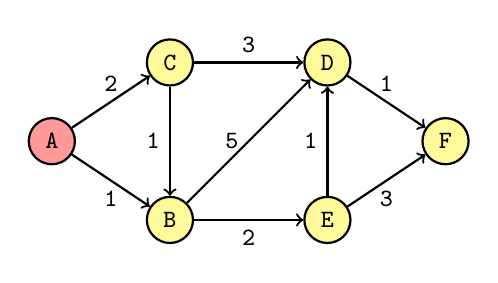
\begin{tikzpicture}[
    thick,
    font=\ttfamily\bfseries\small
]
\tikzset{
    mynode/.style = {circle, draw=black, align=center,fill=yellow!40},
    mynoder/.style = {circle, draw=black, align=center,fill=red!40},
    edgen/.style = {->,thick},
    edger/.style = {->,ultra thick,red}
}
\node[mynoder] at (0.0,1.0) (a) {A};
\node[mynode]  at (1.5,0.0) (b) {B};
\node[mynode]  at (1.5,2.0) (c) {C};
\node[mynode]  at (3.5,2.0) (d) {D};
\node[mynode]  at (3.5,0.0) (e) {E};
\node[mynode]  at (5.0,1.0) (f) {F};
\draw[edgen] (a) edge node[below] {1} (b);
\draw[edgen] (a) edge node[above] {2} (c);
\draw[edgen] (c) edge node[left] {1} (b);
\draw[edgen] (c) edge node[above] {3} (d);
\draw[edgen] (b) edge node[left] {5} (d);
\draw[edgen] (b) edge node[below] {2} (e);
\draw[edgen] (e) edge node[below] {3} (f);
\draw[edgen] (e) edge node[left] {1} (d);
\draw[edgen] (d) edge node[above] {1} (f);
\end{tikzpicture}
\column{0.48\textwidth}
\begin{tabular}{c|ccccccc}
 & & \texttt{\,A\,} & \texttt{\,B\,} & \texttt{\,C\,} & \texttt{\,E\,} & \texttt{\,D\,} & \texttt{\,F\,} \\
\hline
\texttt{A} & 0 & \alert{0} & \xout{0} & \xout{0} & \xout{0} & \xout{0} & \xout{0} \\
\texttt{B} & $\infty$ & 1 & \alert{1} & \xout{1} & \xout{1} & \xout{1} & \xout{1} \\
\texttt{C} & $\infty$ & 2 & 2 & \alert{2} & \xout{2} & \xout{2} & \xout{2} \\
\texttt{D} & $\infty$ & $\infty$ & 6 & 5 & 4 & \alert{4} & \xout{4} \\
\texttt{E} & $\infty$ & $\infty$ & 3 & 3 & \alert{3} & \xout{3} & \xout{3} \\
\texttt{F} & $\infty$ & $\infty$ & $\infty$ & $\infty$ & 6 & 5 & \alert{5} \\
\end{tabular}

\end{columns}

\smallskip
\BB{Spiegazione}
\BIL
\item Ogni colonna contiene lo stato del vettore $d$ all'inizio di ogni ripetizione del ciclo $\mathbf{while}\ \mathbf{not}\ S.\textsf{isEmpty}()$
\item Ogni riga $v$ rappresenta l'evoluzione dello stato dell'elemento $d[v]$
\item La legenda delle colonne rappresenta il nodo che viene estratto
\EIL
\end{frame}

\begin{frame}{Dijkstra}

\begin{block}{Correttezza per pesi positivi}
\BIL 
\item Ogni nodo viene estratto una e una sola volta
\item Al momento dell'estrazione la sua distanza è minima    
\EIL
\end{block}

\bigskip
\BB{Per induzione sul numero $k$ di nodi estratti}

\BIL
\item Caso base: vero perchè $d[s]=0$ e non ci sono lunghezze negative
\item Ipotesi induttiva: vero per i primi $k-1$ nodi
\item Passo induttivo: quando viene estratto il $k$-esimo nodo $u$:
  \BI
  \item La sua distanza $d[u]$ dipende dai $k-1$ nodi già estratti
  \item Non può dipendere dai nodi ancora da estrarre, che ha distanza $\geq d[u]$
  \item Quindi $d[u]$ è minimo e $u$ non verrà più re-inserito, perchè non ci sono distanze negative
\EI
\EIL

\end{frame}

\begin{frame}{Dijkstra, 1959 -- Coda con priorità basata su vettore}


\BB{Costo computazionale}

\begin{columns}
\column{0.45\textwidth}

\begin{tabular}{|l|l|l|}
\hline
Riga & Costo & Ripet. \\\hline
(1) & $O(n)$ & 1 \\\hline
(2) & $O(n)$ & $O(n)$ \\\hline
(3) & $O(1)$ & $O(n)$ \\\hline
(4) & $O(1)$ & $O(m)$ \\\hline
\end{tabular}

\medskip
Costo totale: \alert{$O(n^2)$}

\column{0.5\textwidth}
\vspace{-12pt}
\tiny
\begin{Procedure}
\caption[A]{\textsf{shortestPath}($\Graph\ G,\ \Node\ s$)}
\lnlset{line:shortest-init}{(1)}\alert{$\Heap\ S = \textsf{PriorityQueue}(); S.\textsf{insert}(s, 0)$}\;
\While{\NOT\ $S.\textsf{isEmpty}()$}
{
  \lnlset{line:shortest-remove}{(2)}\alert{$u = S.\textsf{deleteMin}()$}\;
  $b[u] = \FALSE$\;
  \ForEach{$v \in G.\textsf{adj}(u)$}
  {
    \If{$d[u] +G.w(u,v) < d[v]$}
    {
      \eIf{\NOT\ $b[v]$}
      {
        \lnlset{line:shortest-add}{(3)}\alert{$S.\textsf{insert}(v, d[u]+G.w(u,v))$}\;
        $b[v] = \TRUE$\;
      }
      {
        \lnlset{line:shortest-update}{(4)}\alert{$S.\textsf{decrease}(v, d[u]+G.w(u,v))$}
      }
      $T[v] = u$\;
      $d[v] = d[u] + G.w(u,v)$\;
    }
  }
}
\Return $(T,d)$
\end{Procedure}
\end{columns}



\end{frame}

\subsection{Johnson}

\begin{frame}{Johnson, 1977 -- Coda con priorità basata su heap binario}


\BB{Costo computazionale}

\begin{columns}
\column{0.45\textwidth}

\begingroup
\renewcommand*{\arraystretch}{1.2}
\begin{tabular}{|l|l|l|}
\hline
Riga & Costo & Ripet. \\\hline
(1) & $O(n)$ & 1 \\\hline
(2) & $O(\log n)$ & $O(n)$ \\\hline
(3) & $O(\log n)$ & $O(n)$ \\\hline
(4) & $O(\log n)$ & $O(m)$ \\\hline
\end{tabular}
\endgroup

\medskip
Costo totale: \alert{$O(m \log n)$}

\medskip
Heap binario introdotto nel 1964

\column{0.5\textwidth}
\vspace{-12pt}
\tiny
\begin{Procedure}
\caption[A]{\textsf{shortestPath}($\Graph\ G,\ \Node\ s$)}
\lnlset{line:shortest-init}{(1)}\alert{$\Heap\ S = \textsf{PriorityQueue}(); S.\textsf{insert}(s, 0)$}\;
\While{\NOT\ $S.\textsf{isEmpty}()$}
{
  \lnlset{line:shortest-remove}{(2)}\alert{$u = S.\textsf{deleteMin}()$}\;
  $b[u] = \FALSE$\;
  \ForEach{$v \in G.\textsf{adj}(u)$}
  {
    \If{$d[u] +G.w(u,v) < d[v]$}
    {
      \eIf{\NOT\ $b[v]$}
      {
        \lnlset{line:shortest-add}{(3)}\alert{$S.\textsf{insert}(v, d[u]+G.w(u,v))$}\;
        $b[v] = \TRUE$\;
      }
      {
        \lnlset{line:shortest-update}{(4)}\alert{$S.\textsf{decrease}(v, d[u]+G.w(u,v))$}
      }
      $T[v] = u$\;
      $d[v] = d[u] + G.w(u,v)$\;
    }
  }
}
\Return $(T,d)$
\end{Procedure}
\end{columns}



\end{frame}

\subsection{Fredman-Tarjan}


\begin{frame}{Fredman-Tarjan, 1987 -- Heap di Fibonacci}


\BB{Costo computazionale}

\begin{columns}
\column{0.45\textwidth}

\begingroup
\renewcommand*{\arraystretch}{1.2}
\begin{tabular}{|l|l|l|}
\hline
Riga & Costo & Ripet. \\\hline
(1) & $O(n)$ & 1 \\\hline
(2) & $O(\log n)$ & $O(n)$ \\\hline
(3) & $O(\log n)$ & $O(n)$ \\\hline
(4) & $O(1)^{(*)}$ & $O(m)$ \\\hline
\end{tabular}
\endgroup

\medskip
Costo: \alert{$O(m + n \log n)$}

\medskip
(*) Costo ammortizzato

\column{0.5\textwidth}
\vspace{-12pt}
\tiny
\begin{Procedure}
\caption[A]{\textsf{shortestPath}($\Graph\ G,\ \Node\ s$)}
\lnlset{line:shortest-init}{(1)}\alert{$\Heap\ S = \textsf{PriorityQueue}(); S.\textsf{insert}(s, 0)$}\;
\While{\NOT\ $S.\textsf{isEmpty}()$}
{
  \lnlset{line:shortest-remove}{(2)}\alert{$u = S.\textsf{deleteMin}()$}\;
  $b[u] = \FALSE$\;
  \ForEach{$v \in G.\textsf{adj}(u)$}
  {
    \If{$d[u] +G.w(u,v) < d[v]$}
    {
      \eIf{\NOT\ $b[v]$}
      {
        \lnlset{line:shortest-add}{(3)}\alert{$S.\textsf{insert}(v, d[u]+G.w(u,v))$}\;
        $b[v] = \TRUE$\;
      }
      {
        \lnlset{line:shortest-update}{(4)}\alert{$S.\textsf{decrease}(v, d[u]+G.w(u,v))$}
      }
      $T[v] = u$\;
      $d[v] = d[u] + G.w(u,v)$\;
    }
  }
}
\Return $(T,d)$
\end{Procedure}
\end{columns}

\end{frame}

\subsection{Bellman-Ford-Moore}

%-------------------------------------------------------------------------
\begin{frame}{Bellman-Ford, Moore, 1958 -- Coda}

\BB{Storia}
\BI
\item Proposto da Alfonso Shimbel nel 1955
\item Pubblicato da Lester Ford, Jr. nel 1956
\item Pubblicato da Moore nel 1957
\item Pubblicato da Richard Bellman nel 1958
\item Noto come Bellman-Ford, o Bellman-Ford-Moore
\EI

\bigskip
\BB{Note}
\BI
\item Computazionalmente più pesante di Dikstra
\item Funziona anche con archi di peso negativo
\EI

\end{frame}


%-------------------------------------------------------------------------
\begin{frame}{Bellman-Ford, Moore, 1958 -- Coda}

\smallskip
\BB{Linea (1): Inizializzazione}
\BI
\item Viene creata una coda di dimensione $n$
\item Costo computazionale: $O(n)$
\EI

\vspace{-18pt}
\begin{columns}
\column{0.0001\textwidth}
\column{0.97\textwidth}
\small
\begin{Procedure}
\caption[A]{$(\INTARRAY, \INTARRAY)$ \textsf{shortestPath}($\Graph\ G,\ \Node\ s$)}
\lnlset{line:shortest-init}{(1)}\alert{$\Queue\ S = \queueconstructor(); S.\textsf{enqueue}(s)$}\;
\While{\NOT\ $S.\setempty()$}
{
  \lnlset{line:shortest-remove}{(2)}$\INTEGER\ u = S.\textsf{extract}()$\;
  $b[u] = \FALSE$\;
  \ForEach{$v \in G.\adj(u)$}
  {
    \If{$d[u] +G.w(u,v) < d[v]$}
    {
      [...]
    }
  }
}
\Return $(T,d)$
\end{Procedure}
\end{columns}




\end{frame}


%-------------------------------------------------------------------------
\begin{frame}{Bellman-Ford, Moore, 1958 -- Coda}

\smallskip
\BB{Linea (2): Estrazione}
\BI
\item Viene estratto il prossimo elemento della coda
\item Costo computazionale: $O(1)$
\EI

\vspace{-18pt}
\begin{columns}
\column{0.0001\textwidth}
\column{0.97\textwidth}
\small
\begin{Procedure}
\caption[A]{$(\INTARRAY, \INTARRAY)$ \textsf{shortestPath}($\Graph\ G,\ \Node\ s$)}
\lnlset{line:shortest-init}{(1)}$\Queue\ S = \queueconstructor(); S.\textsf{enqueue}(s)$\;
\While{\NOT\ $S.\setempty()$}
{
  \lnlset{line:shortest-remove}{(2)}\alert{$u = S.\textsf{dequeue}()$}\;
  $b[u] = \FALSE$\;
  \ForEach{$v \in G.\adj(u)$}
  {
    \If{$d[u] +G.w(u,v) < d[v]$}
    {
      [...]
    }
  }
}
\Return $(T,d)$
\end{Procedure}
\end{columns}

\end{frame}

%-------------------------------------------------------------------------
\begin{frame}{Bellman-Ford, Moore, 1958 -- Coda}

\smallskip
\BB{Linea (3): Inserimento in coda}
\BI
\item Si inserisce l'indice $v$ in coda
\item Costo computazionale: $O(1)$
\EI

\vspace{-18pt}
\begin{columns}
\column{0.0001\textwidth}
\column{0.97\textwidth}
\small
\begin{Procedure}
\caption[A]{$(\INTARRAY, \INTARRAY)$ \textsf{shortestPath}($\Graph\ G,\ \Node\ s$)}
[...]\;
    \If{$d[u] +G.w(u,v) < d[v]$}
    {
      \eIf{\NOT\ $b[v]$}
      {
        \lnlset{line:shortest-add}{(3)}\alert{$S.\textsf{enqueue}(v)$}\;
        $b[v] = \TRUE$\;
      }
      {
        \lnlset{line:shortest-update}{(4)}\% Azione da intraprendere nel caso $v$ sia già presente in $S$
      }
      $T[v] = u$\;
      $d[v] = d[u] + G.w(u,v)$\;
    }
[...]\;
\end{Procedure}
\end{columns}

\end{frame}

%-------------------------------------------------------------------------
\begin{frame}{Bellman-Ford, Moore, 1958 -- Coda}

\smallskip
\BB{Linea (4): Azione da intraprendere nel caso $v$ sia già presente in $S$}
\BI
\item Sezione non necessaria
\EI

\vspace{-18pt}
\begin{columns}
\column{0.0001\textwidth}
\column{0.97\textwidth}
\small
\begin{Procedure}
\caption[A]{$(\INTARRAY, \INTARRAY)$ \textsf{shortestPath}($\Graph\ G,\ \Node\ s$)}
[...]\;
    \If{$d[u] +G.w(u,v) < d[v]$}
    {
      \If{\NOT\ $b[v]$}
      {
        \lnlset{line:shortest-add}{(3)}$S.\textsf{enqueue}(v)$\;
        $b[v] = \TRUE$\;
      }
      $T[v] = u$\;
      $d[v] = d[u] + G.w(u,v)$\;
    }
[...]\;
\end{Procedure}
\end{columns}

\end{frame}



\begin{frame}{Bellman-Ford, Moore, 1958 -- Coda}

\begin{columns}[T]
\column{0.45\textwidth}
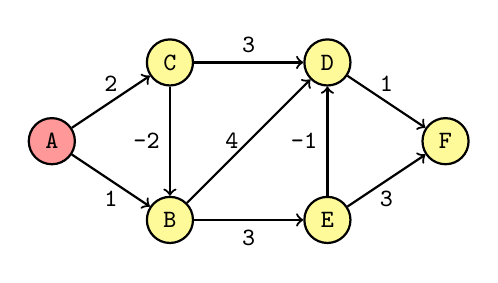
\begin{tikzpicture}[
    thick,
    font=\ttfamily\bfseries\small
]
\tikzset{
    mynode/.style = {circle, draw=black, align=center,fill=yellow!40},
    mynoder/.style = {circle, draw=black, align=center,fill=red!40},
    edgen/.style = {->,thick},
    edger/.style = {->,ultra thick,red}
}
\node[mynoder] at (0.0,1.0) (a) {A};
\node[mynode]  at (1.5,0.0) (b) {B};
\node[mynode]  at (1.5,2.0) (c) {C};
\node[mynode]  at (3.5,2.0) (d) {D};
\node[mynode]  at (3.5,0.0) (e) {E};
\node[mynode]  at (5.0,1.0) (f) {F};
\draw[edgen] (a) edge node[below] {1} (b);
\draw[edgen] (a) edge node[above] {2} (c);
\draw[edgen] (c) edge node[left] {-2} (b);
\draw[edgen] (c) edge node[above] {3} (d);
\draw[edgen] (b) edge node[left] {4} (d);
\draw[edgen] (b) edge node[below] {3} (e);
\draw[edgen] (e) edge node[below] {3} (f);
\draw[edgen] (e) edge node[left] {-1} (d);
\draw[edgen] (d) edge node[above] {1} (f);
\end{tikzpicture}
\column{0.45\textwidth}
\BI
\item La prima riga contiene l'elemento estratto dalla coda
\item L'ultima riga contiene lo stato della coda
\EI
\end{columns}

\small
\bigskip
\begin{tabular}{c||c|c|cc|ccc|ccc|c|c}
&          & \texttt{A} & \texttt{B} & \texttt{C} & \texttt{D} & \texttt{E} & \texttt{B} & \texttt{F} & \texttt{D} & \texttt{E} & \texttt{D} & \texttt{F} \\\hline\hline
\texttt{A} & 0        & 0        & 0        & 0        & 0 & 0 & 0 & 0 & 0 & 0 & 0 & 0 \\ 
\texttt{B} & $\infty$ & 1        & 1        & 0        & 0 & 0 & 0 & 0 & 0 & 0 & 0 & 0 \\ 
\texttt{C} & $\infty$ & 2        & 2        & 2        & 2 & 2 & 2 & 2 & 2 & 2 & 2 & 2 \\ 
\texttt{D} & $\infty$ & $\infty$ & 5        & 5        & 5 & 3 & 3 & 3 & 3 & 2 & 2 & 2 \\ 
\texttt{E} & $\infty$ & $\infty$ & 4        & 4        & 4 & 4 & 3 & 3 & 3 & 3 & 3 & 3 \\ 
\texttt{F} & $\infty$ & $\infty$ & $\infty$ & $\infty$ & 6 & 5 & 5 & 5 & 4 & 4 & 3 & 3 \\\hline
$S$ & \texttt{~A~} & \texttt{BC~} & \texttt{CDE} & \texttt{DEB} & \texttt{EBF} & \texttt{BFD} & \texttt{FDE} & \texttt{DE~} & \texttt{~E~} & \texttt{~D~} & \texttt{~F~} &  \\ 
\end{tabular}

\end{frame}

\begin{frame}{Bellman-Ford, Moore, 1958 -- Coda}

\BB{Passata - definizione ricorsiva}
\BIL
\item Per $k=0$, la zeresima passata consiste nell'estrazione del nodo $s$ dalla coda $S$;
\item Per $k>0$, la $k$-esima passata consiste nell'estrazione di tutti i nodi 
presenti in $S$ al termine della passata $k-1$-esima.
\EIL

\BB{Correttezza -- intuizione}
\BIL
\item Al termine della passata $k$, i vettori $T$ e $d$ descrivono i cammini minimi di
lunghezza al più $k$ 
\item Al termine della passata $n-1$, i vettori $T$ e $d$ descrivono i cammini minimi
(di lunghezza al più $n-1$)
\EIL

\end{frame}

\begin{frame}{Bellman-Ford, Moore, 1958 -- Coda}


\BB{Costo computazionale}

\begin{columns}
\column{0.45\textwidth}

\begingroup
\renewcommand*{\arraystretch}{1.2}
\begin{tabular}{|l|l|l|}
\hline
Riga & Costo & Ripet. \\\hline
(1) & $O(1)$ & 1 \\\hline
(2) & $O(1)$ & $O(n^2)$ \\\hline
(3) & $O(1)$ & $O(nm)$ \\\hline
\end{tabular}
\endgroup

\medskip
Costo: \alert{$O(nm)$}

\medskip
Ogni nodo può essere inserito ed estratto al massimo $n-1$ volte

\column{0.5\textwidth}
\vspace{-12pt}
\tiny
\begin{Procedure}
\caption[A]{$(\INTARRAY, \INTARRAY)$ \textsf{shortestPath}($\Graph\ G,\ \Node\ s$)}
\lnlset{line:shortest-init}{(1)}\alert{$\Queue\ S = \textsf{Queue}(); S.\textsf{enqueue}(s)$}\;
\While{\NOT\ $S.\textsf{isEmpty}()$}
{
  \lnlset{line:shortest-remove}{(2)}\alert{$u = S.\textsf{dequeue}()$}\;
  $b[u] = \FALSE$\;
  \ForEach{$v \in G.\textsf{adj}(u)$}
  {
    \If{$d[u] +G.w(u,v) < d[v]$}
    {
      \If{\NOT\ $b[v]$}
      {
        \lnlset{line:shortest-add}{(3)}\alert{$S.\textsf{enqueue}(v, d[u]+G.w(u,v))$}\;
        $b[v] = \TRUE$\;
      }
      $T[v] = u$\;
      $d[v] = d[u] + G.w(u,v)$\;
    }
  }
}
\Return $(T,d)$
\end{Procedure}
\end{columns}

\end{frame}

\subsection{Casi speciali -- DAG}

\begin{frame}{Cammini minimi su DAG}

\BB{Osservazione}
\BIL
\item I cammini minimi in un DAG sono sempre ben definiti; anche in presenza di
pesi negativi, non esistono cicli negativi
\item E' possibile rilassare gli archi in ordine topologico, una volta sola. 
Non essendoci cicli, non c'è modo di tornare su un nodo già visitato e 
abbassare il valore del suo campo $d$
\EIL

\bigskip
\BB{Algoritmo}
\BIL
\item Si utilizza l'ordinamento topologico
\EIL

\end{frame}

\begin{frame}{Cammini minimi su DAG}

\vspace{-24pt}
\begin{columns}
\column{0.0001\textwidth}
\column{0.97\textwidth}
\begin{Procedure}
\caption[A]{$(\INTARRAY, \INTARRAY)$ \textsf{shortestPath}($\Graph\ G,\ \Node\ s$)}
$\INTEGER[\,]\ d = \NEW\ \INTEGER[1 \mldots G.n]$\REMR{$d[u]$ è la distanza da $s$ a $u$ }
$\INTEGER[\,]\ T = \NEW\ \INTEGER[1 \mldots G.n]$\REMR{$T[u]$ è il padre di $u$ nell'albero $T$ }
\ForEach{$u \in G.\VV()-\{s\}$}
{
  $T[u] = \Nil$; $d[u] = +\infty$\; 
}
$T[s] = \Nil$; $d[s] = 0$\; 
$\Stack\ S = \textsf{topsort}(G)$\;
\While{\NOT\ $S.\textsf{isEmpty}()$}
{
  $u = S.\textsf{pop}()$\;
  \ForEach{$v \in G.\textsf{adj}(u)$}
  {
    \If{$d[u] +G.w(u,v) < d[v]$}
    {
      $T[v] = u$\;
      $d[v] = d[u] + G.w(u,v)$\;
    }
  }
}
\Return $(T,d)$
\end{Procedure}
\end{columns}

\end{frame}

\begin{frame}{Riassunto}

\BB{Complessità: quale preferire?}

\medskip
\begingroup
\renewcommand*{\arraystretch}{1.2}
\begin{tabular}{|l|l|P{5cm}|}
\hline
Dijkstra & $O(n^2)$ & Pesi positivi, grafi densi \\\hline
Johnson & $O(m \log n)$ & Pesi positivi, grafi sparsi \\\hline
Fredman-Tarjan & $O(m + n \log n)$ & Pesi positivi, grafi densi, dimensioni molto grandi  \\\hline
Bellman-Ford & $O(mn)$ & Pesi negativi \\\hline
  & $O(m+n)$ & DAG \\\hline
BFS & $O(m+n)$ & Senza pesi \\\hline
\end{tabular}
\endgroup

\end{frame}


\section{Cammini minimi, sorgente multipla}

\begin{frame}{Cammini minimi, sorgente multipla}

\BB{Possibili soluzioni}

\medskip
\begingroup
\renewcommand*{\arraystretch}{1.2}
\small
\begin{tabular}{|P{2.3cm}|P{2.6cm}|P{5.8cm}|}
\hline
\textbf{Input} & \textbf{Complessità} & \textbf{Approccio} \\\hline
Pesi positivi, grafo denso & $O(n \cdot n^2)$ & Applicazione ripetuta dell'algoritmo di Dijkstra \\\hline
Pesi positivi, grafo sparso & $O(n \cdot (m \log n))$ & Applicazione ripetuta dell'algoritmo di Johnson \\\hline
Pesi negativi & $O(n \cdot nm)$ & Applicazione ripetuta di Bellman-Ford, \alert{sconsigliata} \\\hline
Pesi negativi, grafo denso & $O(n^3)$ & Algoritmo di \alert{Floyd e Warshall} \\\hline
Pesi negativi, grafo sparso & $O(nm \log n)$ & Algoritmo di \alert{Johnson per sorgente multipla} \\\hline
\end{tabular}
\endgroup

\end{frame}

\subsection{Floyd-Warshall}

\begin{frame}{Floyd-Warshall, 1962}

\begin{block}{Cammini minimi $k$-vincolati}
Sia $k$ un valore in $\{0,\ldots,n\}$. Diciamo che un cammino 
$p_{xy}^k$ è un \alert{cammino minimo $k$-vincolato} fra $x$ e $y$ 
se esso ha il costo minimo fra tutti i cammini fra $x$ e $y$ 
che non passano per nessun vertice in $v_{k+1}, \ldots, v_n$
($x$ e $y$ sono esclusi dal vincolo).
\end{block}

\bigskip
\BB{Note}
Assumiamo (come abbiamo sempre fatto) che esista un ordinamento fra i nodi
del grafo $v_1, v_2, \ldots, v_n$.

\bigskip
\BB{Domande}
\BIL
\item A cosa corrisponde $p^0_{xy}$?
\item A cosa corrisponde $p^n_{xy}$?
\EIL

\end{frame}

\begin{frame}{Floyd-Warshall, 1962}

\begin{block}{Distanza $k$-vincolata}
Denotiamo con $d^k[x][y]$ il costo totale del cammino minimo $k$-vincolato
fra $x$ e $y$, se esiste.
\[
  d^k[x][y]) = \begin{cases}
    w(p_{xy}^k) & \textrm{se esiste $p_{xy}^k$}\\
    +\infty & \textrm{altrimenti}
  \end{cases}
\]
\end{block}

\bigskip
\BB{Domande}
\BIL
\item A cosa corrisponde $d^0[x][y]$?
\item A cosa corrisponde $d^n[x][y]$?
\EIL

\end{frame}

\begin{frame}{Floyd-Warshall, 1962}

\BB{Formulazione ricorsiva}
\[
  d^k[x][y]) = \begin{cases}
    w(x,y) & k = 0 \\
    \pause \min({\color{blue}{d^{k-1}[x][y]}}, {\color{red} d^{k-1}[x][k] + d^{k-1}[k][y]}) & k>0
  \end{cases}
\]

\bigskip
\BB{Esempio}

\begin{columns}[T]
\column{0.4\textwidth}
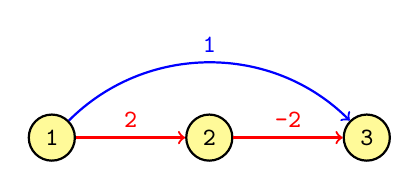
\begin{tikzpicture}[
    thick,
    font=\ttfamily\bfseries\small
]
\tikzset{
    mynode/.style = {circle, draw=black, align=center,fill=yellow!40},
    mynoder/.style = {circle, draw=black, align=center,fill=red!40},
    edgen/.style = {->,thick},
    edger/.style = {->,ultra thick,red}
}
\node[mynode] at (0.0,0.0) (a) {1};
\node[mynode] at (2.0,0.0) (b) {2};
\node[mynode] at (4.0,0.0) (c) {3};
\draw[edgen,red] (a) edge node[above] {2} (b);
\draw[edgen,red] (b) edge node[above] {-2} (c);
\draw[edgen,blue] (a) edge[bend left=45] node[above] {1} (c);
\end{tikzpicture}
\column{0.55\textwidth}
\begin{align*}
d^0[1][3] &= 1 \\
d^1[1][3] &= 1 \\
d^2[1][3] &= \min(d^1[1][3], d^1[1][2]+d^2[2][3]) \\
          &= \min(1,0) = 0
\end{align*}

\end{columns}

\end{frame}

\begin{frame}{Floyd-Warshall, 1962}

\BB{Matrice dei padri}
Oltre a definire la matrice $d$, calcoliamo una matrice $T$ dove $T[x][y]$ rappresenta il predecessore
di $y$ nel cammino più breve da $x$ a $y$.

\bigskip
\BB{Esempio}

\begin{columns}[T]
\column{0.4\textwidth}
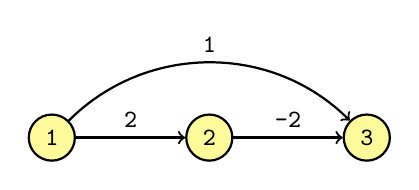
\begin{tikzpicture}[
    thick,
    font=\ttfamily\bfseries\small
]
\tikzset{
    mynode/.style = {circle, draw=black, align=center,fill=yellow!40},
    mynoder/.style = {circle, draw=black, align=center,fill=red!40},
    edgen/.style = {->,thick},
    edger/.style = {->,ultra thick,red}
}
\node[mynode] at (0.0,0.0) (a) {1};
\node[mynode] at (2.0,0.0) (b) {2};
\node[mynode] at (4.0,0.0) (c) {3};
\draw[edgen] (a) edge node[above] {2} (b);
\draw[edgen] (b) edge node[above] {-2} (c);
\draw[edgen] (a) edge[bend left=45] node[above] {1} (c);
\end{tikzpicture}
\column{0.55\textwidth}
\begin{align*}
T[1][2] &= 1 \\
T[2][3] &= 2 \\
T[1][3] &= 2
\end{align*}
 
\end{columns}


\end{frame}



\begin{frame}{Floyd-Warshall, programmazione dinamica}

\vspace{-6pt}
\begin{Procedure}
\caption[A]{$(\INTARRAY[\,], \INTARRAY[\,])$ \floyd(\Graph\ $G$)}
$\INTARRAY[\,]\ d = \NEW\ \INTEGER[1 \ldots n][1 \ldots n]$\;
$\INTARRAY[\,]\ T = \NEW\ \INTEGER[1 \ldots n][1 \ldots n]$\;
\ForEach{$u,v \in G.\VV()$}{
  $d[u][v] = +\infty$\;
  $T[u][v] = \Nil$\;
}
\ForEach{$u \in G.\VV()$} {
  \ForEach{$v \in G.\adj(u)$} {
    $d[u][v] = G.w(u,v)$\;
    $T[u][v] = u$\;
  }
}
\end{Procedure}
\end{frame}

\begin{frame}{Floyd-Warshall, programmazione dinamica}

\vspace{-6pt}
\begin{Procedure}
\caption[A]{$(\INTARRAY[\,], \INTARRAY[\,])$ \floyd(\Graph\ $G$)}
[...]\;
\For{$k = 1$ \TO\ $G.n$} {
  \ForEach{$u \in G.\VV()$} {
    \ForEach{$v \in G.\VV()$} {
      \If{$d[u][k] + d[k][v] < d[u][v]$}
      {
        $d[u][v] = d[u][k] + d[k][v]$\;
        $T[u][v] = T[k][v]$\;
      }
    }
  }
}
\Return $d$\
\end{Procedure}

\end{frame}

\subsection{Chiusura transitiva}

\begin{frame}{Chiusura transitiva (Algoritmo di Warshall)}

Dato un grafo orientato $G=(V,E)$, la chiusura transitiva $G^*=(V,E^*)$ è il
grafo orientato che contiene un arco $(u,v) \in E^*$ se e solo esiste un cammino da $u$ a $v$ in $G$.

Supponendo di avere il grafo $G$ rappresentato da una matrice di adiacenza $M$, la matrice
$M^n$ rappresenta la matrice di adiacenza di $G^*$.

\bigskip
\BB{Formulazione ricorsiva}
\[
  M^k[x][y]) = \begin{cases}
    M[x][y] & k = 0 \\
    {\color{blue}{M^{k-1}[x][y]}} \vee {\color{red} M^{k-1}[x][k] \wedge M^{k-1}[k][y]}) & k>0
  \end{cases}
\]

\end{frame}


\section{Conclusione}

\begin{frame}{Conclusione}

\BIL
\item Abbiamo visto una panoramica dei più importanti algoritmi per la ricerca
dei cammini minimi
\item Ulteriori possibilità:
\BI
\item A*, un algoritmo che utilizza euristiche per velocizzare la ricerca
\item Algoritmi specializzati per reti stradali
\EI
\EIL

\IG{0.3}{astar.pdf}
\tiny
\url{https://en.wikipedia.org/wiki/A*\_search\_algorithm\#/media/File:Astar\_progress\_animation.gif}

\end{frame}


\end{document}

